\begin{figure}[h!]
\centering
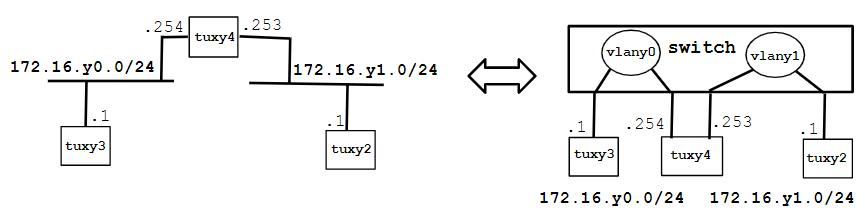
\includegraphics[scale=0.35]{imagens/Exp3.png}
\caption{Arquitetura da Terceira Experiência}
\label{fig:exp3}
\end{figure}

Esta experiência tem como objectivo tornar o tuxy4 num router para possibilitar a comunicação entre o tuxy3 e o tuxy2, através das VLAN's 0 e 1. Para haver comunicação terá de se configurar os endereços IP's das portas ethernet dos tuxy's e as routes que serão usadas.

Os comandos usados para esta experiência podem ser encontrados no Anexo \ref{exp3_steps}.


\subsubsection{Análise dos Logs}

Para adicionar uma route a um dos tuxes é necessário ter três valores: IP da rede a aceder, máscara de bits desse IP e IP da porta a usar como gateway. Para haver ligação entre o tux23 e o tux22, adicionou-se uma route ao tux23 para aceder aos endereços 172.16.21.0/24 a partir do IP 72.16.20.254 (tux24 eth0) e uma route ao tux22 para aceder aos endereços 172.16.20.0/24 a partir do IP 172.16.21.253 (tux24 eth1). Estas routes podem ser vistas na forwarding table, através do comando: route -n.

Com estas routes definidas, é possivel fazer ping, a partir do tux23, a todas as interfaces dos outros tux's (Figura \ref{fig:exp3_tux3_logs}). Também se verifica na figura que a interface eth0 do tux24 enviou 2 pedidos ARP para determinar o endereço MAC da interface eth0 to tux23, enquanto que o tux23 mandou um pedido para saber o endereço MAC da interface eth0 do tux24.

Continuando nas figuras \ref{fig:exp3_tux4_eth0_logs} e \ref{fig:exp3_tux4_eth1_logs}, é possível verificar que existe comunicação entre os tux's 23 e 22, visto que os pings emitidos obtêm uma resposta. Na primeira figura nota-se uma troca de mensagens ARP para o tux23 tomar conhecimento do endereço MAC da interface eth0 to tux24 e vice-versa, enquanto que na segunda figura existe uma troca de mensgens ARP para o tux22 tomar conhecimento do endereço MAC da interface eth1 do tux24 e vice-versa.